\section{Introduction}
As cloud providers allow multi-tenancy in their cloud, 
hostile virtual machines (VMs) can be placed on the same physical machine that 
hosts other regular users. The consequence of this is the 
possibility of cross-VM attacks in which the adversary 
penetrates the hypervisor or uses side-channel to commit 
harms to other VMs. This type of attacks often comes with 
two step: placement and extraction. During placement, 
the attacker exploits the spatiality and/or locality characteristic of 
cloud providers' resource allocation mechanism to place its VM on the 
same physical machine with the victim with a lowest cost. 
Recent work shows that adversary can achieve 
up to 40\% of co-residency in Amazon EC2 cloud with 
just a fews dollars~\cite{ristenpart2009hey}.\\

Many side-channel attacks exploit 
the imperfect resource isolation in virtualization. VMs on a 
same physical machine share local disk, CPU data's cache. 
By listening to the performance of these shared channels, 
VMs can eavesdrop each other. This type of eavesdropping was shown 
be able to extract RSA and AES secret keys, or listen 
to keystroke from the other VM. To commit these attacks, however, 
the attackers have to determine whether they have the 
co-residency with the victim.\\

This lab assignment leverages side-channel monitoring to develop a hard disk based 
co-residency detection. By building a coarse-grained hard disk based covert 
channel, a VM can listen to another VM's disk actions and determine whether they 
are co-resident (phase A). The lab assignment takes a step further by demonstrating that 
an attacker can detect co-residency without having any 
control over the victim but using a remote machine to cause I/O loads 
to the victim and listening to the covert channel (phase B).\\

\section{Design}
The experiment setup consists of two VMs hosted on one physical 
machine and sharing the same local disk (as in Figure~\ref{fig:arch}). The idea behind 
disk based covert channel is that if the two VMs 
simultaneously read/write the local disk, both should see 
a degradation on disk performance; if A idles and B reads/writes 
the disk, B should see a better disk performance compared to the first case. 
The two distinguishable disk performances is sufficient to 
present low/high (0/1) signals and can be used for communication between A and 
B.\\

\begin{figure}[hbtp]
\centering
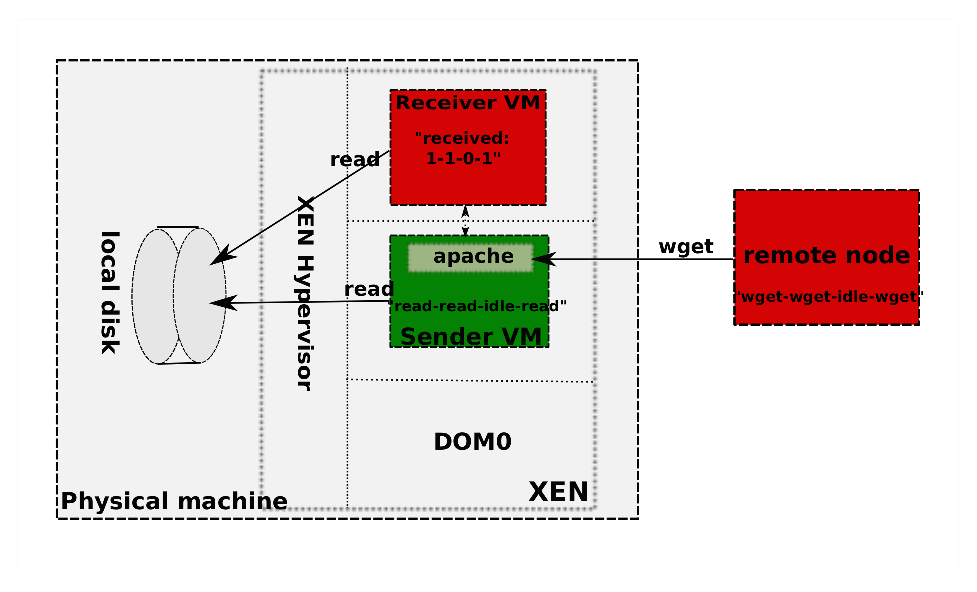
\includegraphics[scale=0.5]{arch.eps}
\caption{Experiment architecture. Sender and receiver (VMs) reside on the 
same physical machine that runs XEN. Both VMs share the same 
local disk. The sender (victim) also runs apache server and allows 
requests from a remote node.}
\label{fig:arch}
\end{figure}

When either sender or receiver reads the local disk, it will 
perceive a high disk reading speed (say N MB/s). When both read the disk 
in the mean time, since the disk is shared, each reader will 
perceive a relatively lower disk reading speed (theoretically N/2 MB/s). 
If the receiver keeps reading the disk and the sender: (i) reads 
the disk when it wants to send "1", (ii) idle when it wants to send 
"0", the receiver will see low disk reading speed when the sender 
sends "1" and high disk reading speed when the sender sends "0". 
By keeping the receiver reading the disk and the sender reads or 
idles, the sender can send "1" or "0" signal to the receiver. This 
is the disk based covert channel.\\

The read actions of sender and receiver, however, have to be 
synchronized for accuracy. While the receiver keeps reading 
the disk, the sender has to maintain the timing for idle/reading 
duration so that the receiver can distinguish between low and 
high period. A possible solution for this timing is to say 
the sender idle or read per X seconds, and the bit rate of the 
covert channel is X bps.\\

For phase B, the idea is to let a remote node to trigger 
I/O loads on the sender and let the receiver detect that. 
In this experiment, the remote node issues wget commands to 
download a large file on the sender. To serve the remote 
host, the sender has to read local disk for the large file and 
this causes I/O loads. In a real attack scenario, the remote host 
trigger the sender at the behest of the attacker, and the triggering 
pattern can be used to detect co-residency. For example, if 
the remote host periodically gets the file and idles, the receiver 
(if co-resides with the sender) should see "1010..." signal.

\section{Implementation}

This experiment runs on Emulab~\cite{white2002integrated} 
machines. One physical node, which is able to do virtualization, 
hosts two XEN VMs instances. The remote node is hosted on a 
separate machine which is able to connect to the other machine.\\

To measure disk reading speed, the experiment uses hdparm, a 
linux built-in command that continuously reads a disk for about 
three seconds and reports the total amount of data read as 
well as the reading speed. The receiver periodically captures 
disk performance using hdparm commands (every 10 seconds). The 
sender receives a "signal" string and sends it using idling or 
reading actions (also every 10 seconds). For example, the sender 
is commanded to send "11010", for every 10 seconds, it performs: 
read (1), read (1), idle (0), read (1), idle (0). The receiver 
sees "11010" correspondingly.\\

For phase B, the sender runs a Apache server and allows the 
remote host to download a large file stored in the local disk. The remote 
host trigger the download to send a "1" signal to the receiver and 
idle to send "0".\\

\section{Result}

The experiment successfully implemented a hard disk based covert channel 
with a bit rate of 6 bps with the accuracy of nearly 100\%. 
The sender is able to send binary signal to the receiver ( Figure ~\ref{fig:sender} and 
~\ref{fig:receiver} ).\\

\begin{figure}[hbtp]
\centering
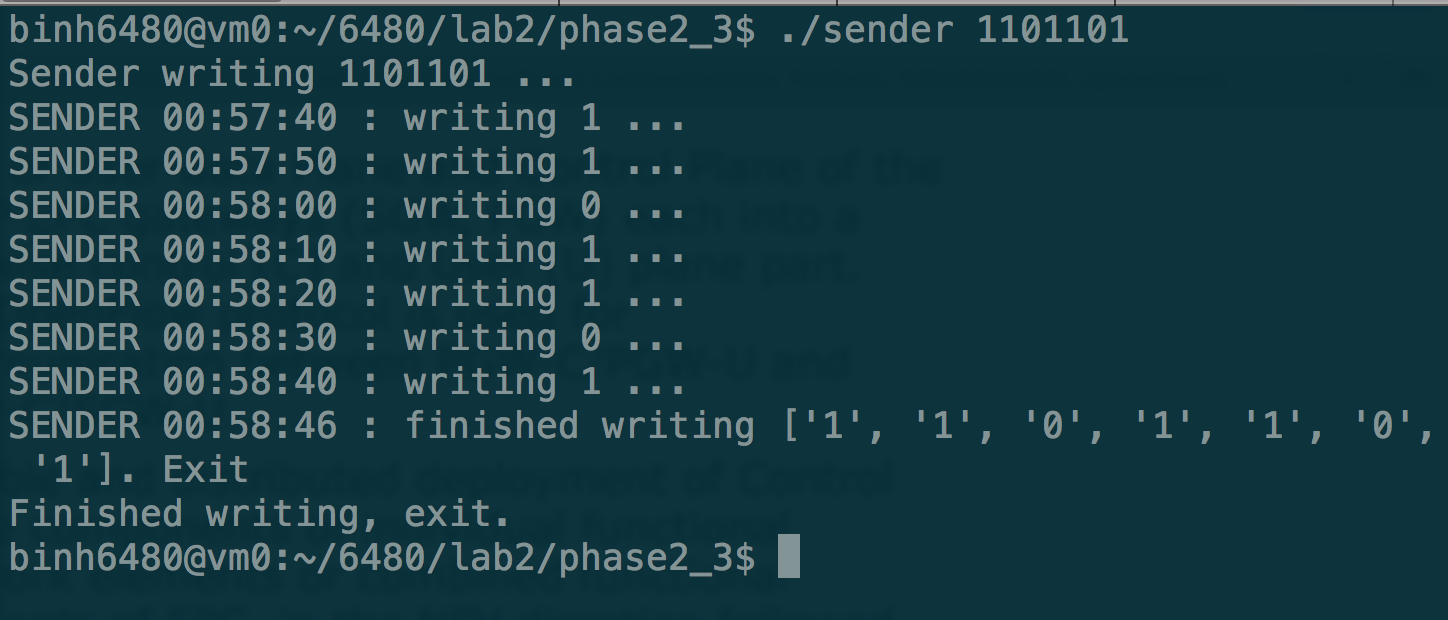
\includegraphics[scale=0.3]{sender.png}
\caption{Sender's screen shoot. Sender sends "1101101" signal, 1 bit every 10 seconds.}
\label{fig:sender}
\end{figure}

\begin{figure}[hbtp]
\centering
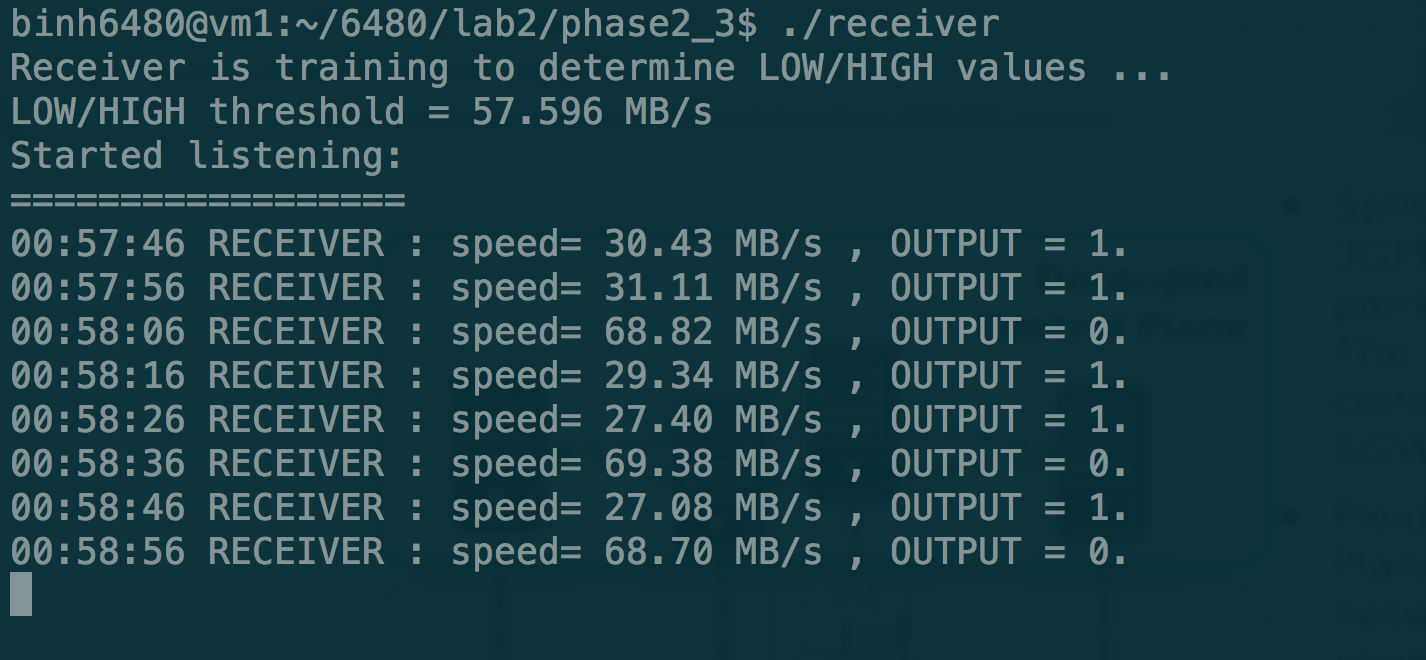
\includegraphics[scale=0.3]{receiver.png}
\caption{Receiver's screen shoot. Receiver receives "1101101" signal, 1 bit every 10 seconds.}
\label{fig:receiver}
\end{figure}

The actual receiver's disk reading speed and received signal are shown in figure ~\ref{fig:speed}. 
The threshold to determine 1 or 0 signal is shown in blue line. This threshold determined 
as 0.85 of the disk speed measured at the time the receiver starts.\\
\begin{figure}[hbtp]
\centering
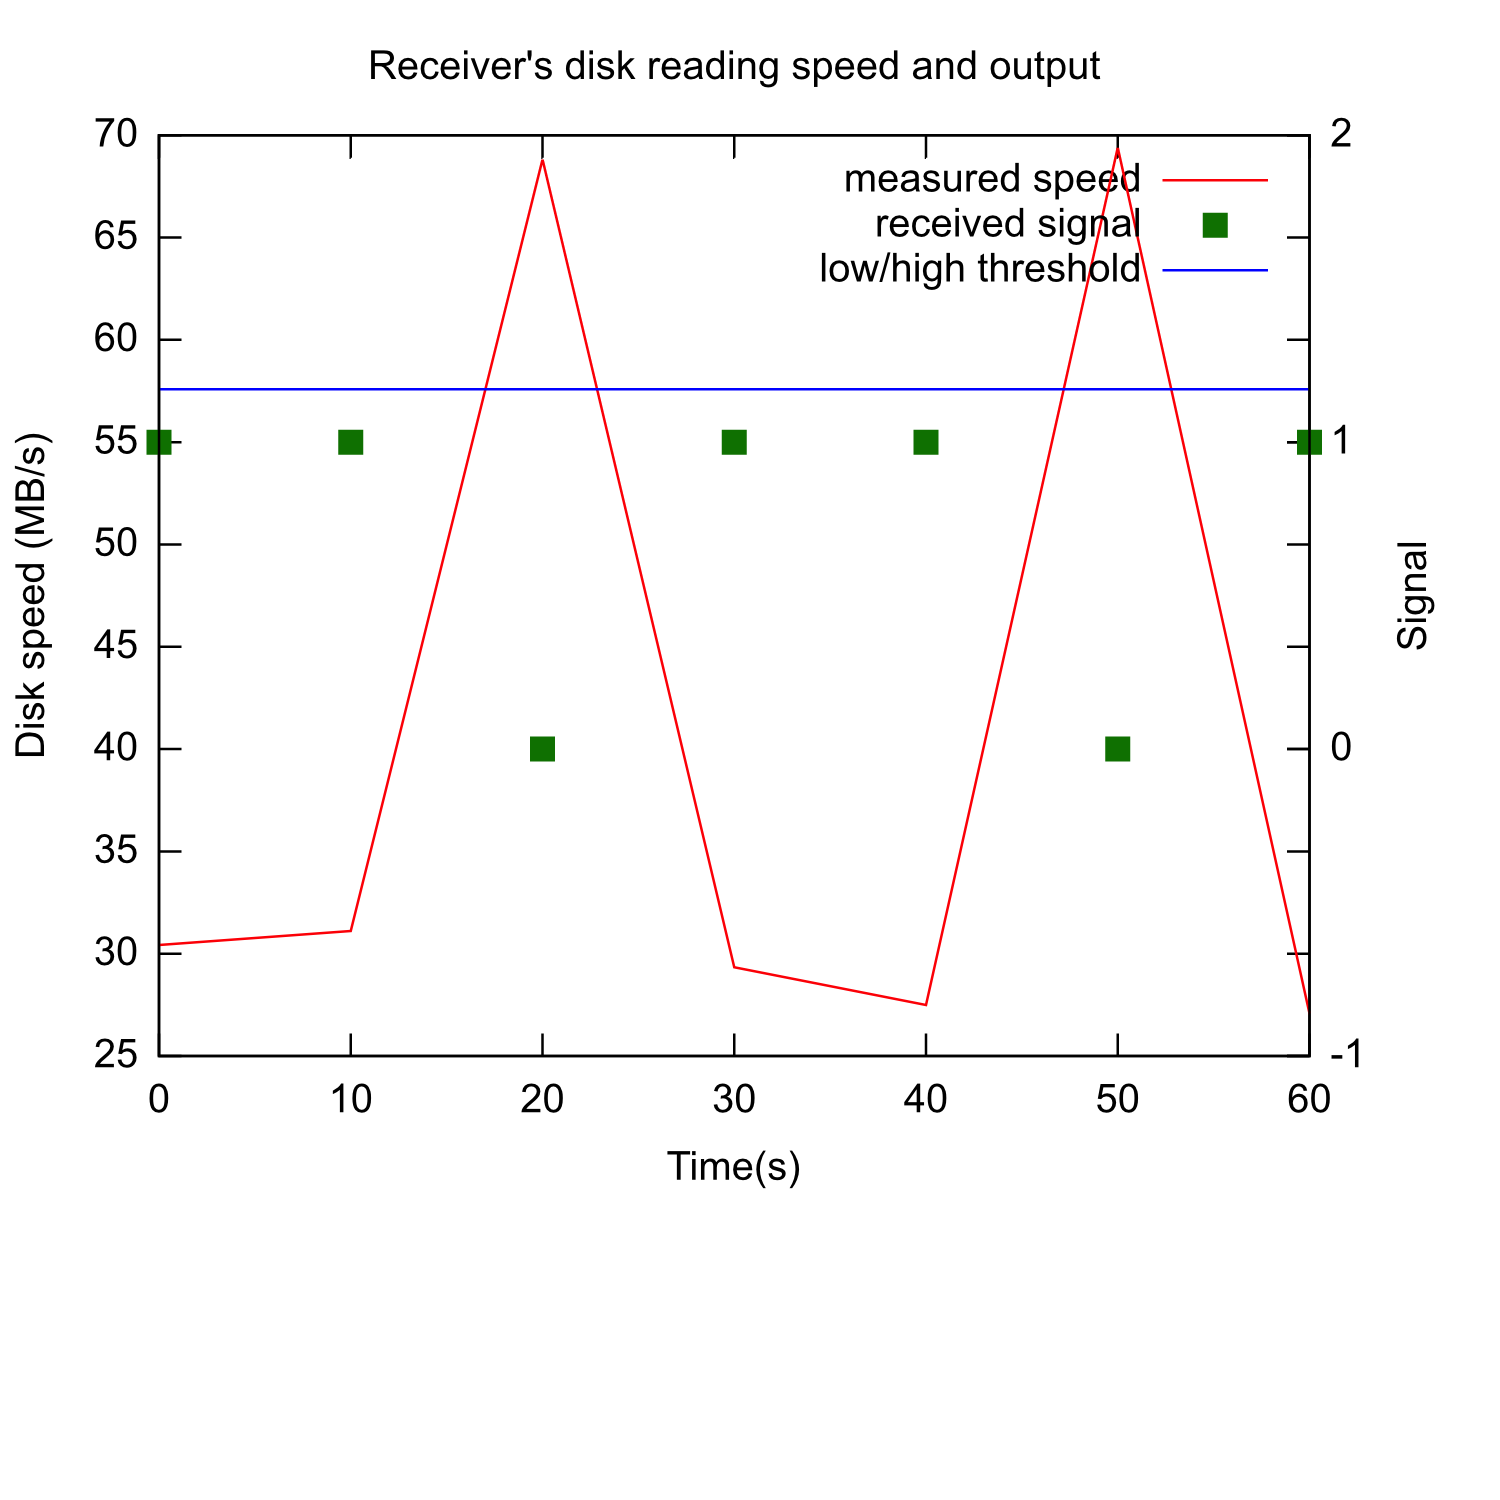
\includegraphics[scale=0.15]{speed.png}
\caption{Receiver's disk reading speed and received signal}
\label{fig:receiver}
\end{figure}

In phase B, the remote host trigger "1010" signal and that signal was picked up by 
the receiver ( Figure ~\ref{fig:remotehost} and ~\ref{fig:receiver-b}). In phase B, 
the remote host downloads a file (or idles) in 60-seconds periods, and the receiver 
reads the disk at the same frequency.\\
\begin{figure}[hbtp]
\centering
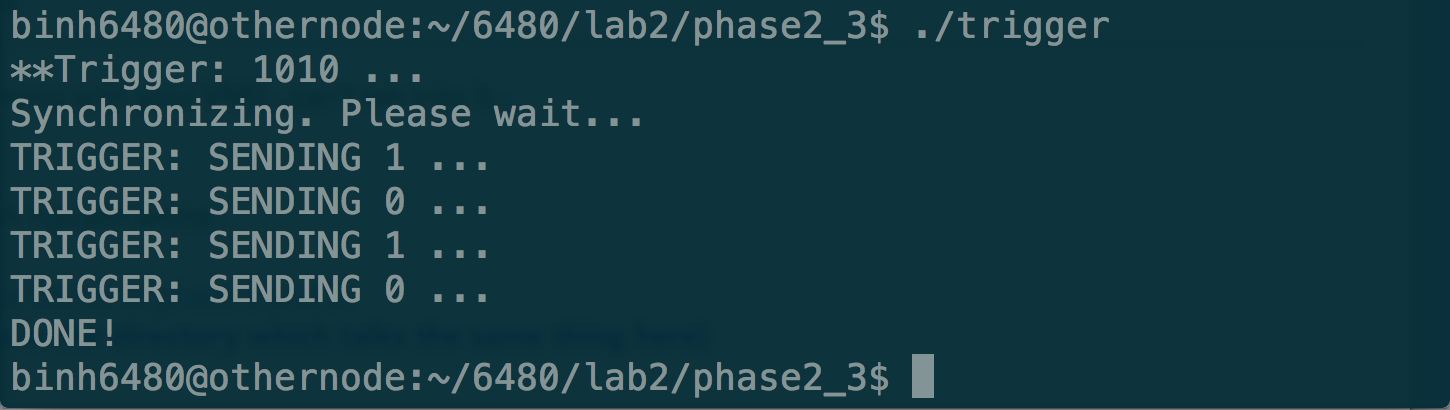
\includegraphics[scale=0.3]{remotehost.png}
\caption{Remote host's screen shoot. Remote host triggers "1010" signal which 
corresponding to "download-idle-download-idle" series of actions.}
\label{fig:remotehost}
\end{figure}

\begin{figure}[hbtp]
\centering
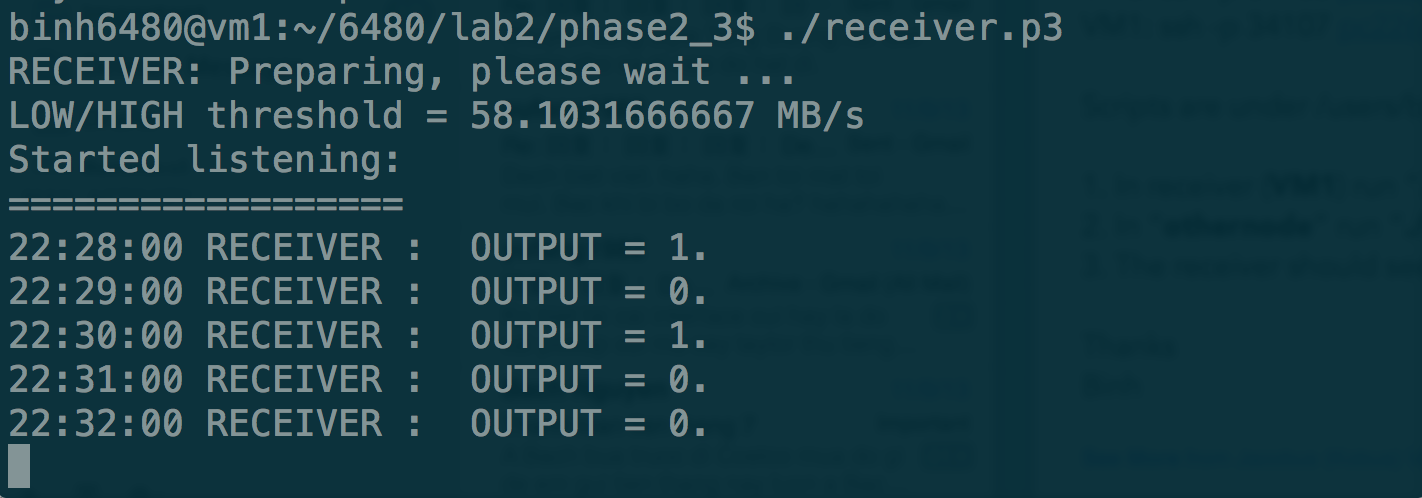
\includegraphics[scale=0.3]{receiver-b.png}
\caption{Receiver's screen shoot in phase B. As the remote host downloads a 
large file from sender, the receiver perceives disk loads and detects 
"1010", the same pattern as the remote host.}
\label{fig:receiver-b}
\end{figure}

\section{Discussion}
Although the experiment successfully implemented a disk based covert channel, 
the channel has some limitations with speed and accuracy. To increase speed 
of the channel, the measurements have to happen more frequently. The result of 
this is less accurate measurements since hard disk is not responsive enough. 
Also, sender and receiver have to be synchronized for better accuracy. Using 
built-in command (hdparm), the experiment was able to implement a highly accurate 
covert channel. However, since hdparm tends to stress test the disk for a 
sufficient amount of time (3s), the covert channel could not be faster than 20 bps.\\

The implementation of phase B is not guaranteed 100\% successful. 
The magnitude of the I/O loads that the remote host causes on the sender depends on (i) the download link's speed 
and (ii) the local disk speed. If the download link's speed is too low 
and/or the local disk speed is too high, then downloading might not be significant 
enough to cause disk performance degradation on the local disk. In the 
experiment, if local disk speed is about 100 MB/s without load, and 
the download speed is about 10 MB/s, the degradation of disk performance is 
less than 10\% (reading speed is always higher than 90 MB/s regardless of 
the downloading).\\

The experiment is done using Python and Bash scripts. 
All the scripts for this lab assignment could be found 
\href{https://github.com/binhqnguyen/cs6480/tree/master/lab2/phase2\_3}{here}. 


